\documentclass{llncs}
\usepackage[margin=1.2in]{geometry}
\usepackage{amsmath,amssymb,amsfonts}
\usepackage{paralist}
\usepackage{graphicx}
\usepackage[usenames,dvipsnames]{xcolor}
\usepackage{listings}
\usepackage{tikz}
\usetikzlibrary{trees}
\usepackage{hyperref}
\bibliographystyle{plain}
\usepackage{wrapfig}

\newcommand\ednote[1]{\typeout{There is still an editor's note!!!}%
  \footnote{EDNOTE: #1}}
\newcommand\edbf[1]{\typeout{There is still an editor's note!!!}%
  \textbf{EDNOTE: #1}}

\def\collapse#1{\textcolor{blue}{\ensuremath{\mathord{\blacktriangleleft}\mathord{#1}
\mathord{\blacktriangleright}}}}


\title{Towards Meaningful Visual Abstraction of Mathematical Notation}
\author{Davide Cervone \and Peter Krautzberger \and Volker Sorge\thanks{This
    work was partially supported by the Alfred P. Sloan Foundation.}}
\institute{MathJax Consortium\\
  \email{dpvc@union.edu, peter.krautzberger@mathjax.org, V.Sorge@cs.bham.ac.uk}
}

\begin{document}
\maketitle
\begin{abstract}
  The large variety of form factors to view web pages and the proliferation of
  the pinch-to-zoom paradigm requires web-content to adapt both font sizes and
  reflow to the requirements of diverse displays and varying magnification. For
  specialist web content, such as mathematical formulas, this is not straight
  forward.  We present a first approach to \emph{responsive equations}, a rendering
  method for MathML that adapts gracefully to small screens. The main idea is to
  reduce the size of equations by abstracting over well-defined parts of formulas
  without obscuring the overall structure of an expression.  We achieve this by
  embedding a semantic structure into the MathML representation underlying the
  rendering process and by collapsing mathematically meaningful sub-expressions.
\end{abstract}

\section{Introduction}
\label{sec:introduction}

Mathematical notation is a corner stone of scientific literature and with more
and more teaching and research material being published in purely electronic
form the electronic display of mathematics has become an important topic.
MathML is the only specialist markup language that has been made part of the
HTML5 and epub3 standard. While this was an important first step, there is still
a long way to go before Mathematical notation becomes a first-class citizen of
the web. Not only is MathML not implemented in all browsers or eBook readers,
forcing developers and content providers to use polyfill solutions like
MathJax~\cite{mathjax} to ensure that content renders consistently across all
platforms, but also the production of mathematical content is still mainly done
in a ``print-first'' manner, giving little thought to the special requirements and
opportunities of electronic display. For example, rigid, tabular layout is
ported directly from print, making it difficult to adjust its display for
different form factors or to exploit features like zooming or panning.

In the past five years, the notion of \emph{responsive web design} (RWD),
introduced in \cite{alistapart} (cf. also \cite{wikiRwd}), has been firmly
established as the dominant design paradigm on the web. RWD aims to dynamically
optimise the layout of a page depending on the capabilities of the end user's
device. The dominating features of RWD are fluid grids for content, flexible
images, and media queries. The related (and older) concept, ``progressive
enhancements'', cf. \cite{progEnh}, leverages feature and (client or
server-side) user-agent detection to enrich the content and rendering.

While RWD offers a firmly established methodology, tools, and workflows for
content such as text, menus, and widgets, the notion of responsive design for
complex content fragments is still in its infancy. This includes responsive
tables \cite{zurbTable} and responsive SVG \cite{smashSvg}. In addition, data
visualisation tools such as d3js allow dynamic rendering of scientific data that
shares some of the traits of responsive design as their dynamic nature enables
developers to modify them on the fly, cf. \cite{safariD3js}.

For MathML, native browser implementations, i.e., Gecko and WebKit, do not yet
provide line-breaking support. Under these circumstances, it might not be
surprising that the notion of responsive rendering has not even been attempted
yet; that is, no new visual concepts have been explored that work with the
fabric of the web, similar to the attempts for tables and SVG. Unlike regular
text that can be easily broken down into paragraphs, sentences, etc., regardless
of their meaning, it is difficult to identify meaningful components in
mathematical formulas without having some information on their actual
semantics. In particular, issues like line breaking, which are straight-forward
for regular text, are difficult for MathML renderers, as large expressions often
have to be broken over multiple lines; this makes the formula hard to read, and
when done badly, can render it practically meaningless.

Consider the example in Table~\ref{tab:example_eq} that was extracted from an
answer on
\href{http://math.stackexchange.com/a/1285149}{math.stackexchange.com},
\cite{mathSE}. Not only is the expression rather large and unwieldy, it also is
given in a pre-formatted tabular style that makes it difficult to decide on both
visually pleasing and mathematically accurate line breaks.  Moreover, some of
the sub-expressions, like the presentation annotation with underbrace or the
wide fration elements, do not lend themselves at all to line
breaking. Consequently display and reading of the expression on a small form
factor can be very awkward.

\begin{table}
  \vspace{-20pt}
  \centering
  \begin{align*}
I_\nu(\nu^{-1},1)
&=\underbrace{\frac{\pi^2}{4}\ln\left(\frac{(1+\nu)^{1+\nu}}{\nu^\nu}
\right)-\frac{7\zeta(3)}{8}\nu}_{\text{Let this be 
C}}+2\int^\frac{1-\nu}{1+\nu}_1\frac{\chi_3(v)}{(1+v)^2}{\rm d}v\\
&=C-\left.\frac{2\chi_3(v)}{1+v}\right|^\frac{1-\nu}{1+\nu}_1+2\int^\frac{1-\nu}
{1+\nu}_1\frac{\chi_2(v)}{v(1+v)}{\rm d}v\\
&=C+(1-\nu)\chi_3\left(\frac{1-\nu}{1+\nu}\right)-\frac{7\zeta(3)}{8}
-\left.{\color{white}{\frac{1}{1}}}2\chi_2(v)\ln(1+v)\right|^\frac{1-\nu}{1+\nu}
_1+\int^\frac{1-\nu}{1+\nu}_1\frac{\ln(1+v)\ln\left(\frac{1+v}{1-v}\right)}{v}{
\rm d}v\\
&=C+(1-\nu)\chi_3\left(\frac{1-\nu}{1+\nu}\right)-\frac{7\zeta(3)}{8}
+2\chi_2\left(\frac{1-\nu}{1+\nu}\right)\ln\left(\frac{1+\nu}{2}\right)+\frac{
\pi^2}{4}\ln{2}\\
&\ \ \ \ 
+\frac{1}{2}\int^\frac{1-\nu}{1+\nu}_1\frac{
\ln^2(1+v)-\ln^2(1-v)+\ln^2\left(\frac{1-v}{1+v}\right)}{v}{\rm d}v
\end{align*}
\caption{Example of mathematics ``in the wild'' taken from \href{http://math.stackexchange.com/a/1285149}{math.stackexchange.com}.}
\label{tab:example_eq}
  \vspace{-20pt}
\end{table}

We currently address these issues within MathJax. In particular, we are
developing new rendering methods for mathematical notation that allow for a
responsive reading experience regardless of platform or form factor. The basic
idea is to enrich standard MathML notation with semantic information computed by
a heuristic interpretation of the Presentation MathML element. We thereby use a
coarse-grained semantic model that aims to capture the maturity of mathematical
notation, including interpretations for purely presentation artefacts, such as
the underbrace in the example above, rather then determining a precise
mathematical semantic that would severely restrict the types of expressions we
could handle. The semantics effectively provide the original MathML expression
with a secondary structure; and while the expression can be rendered as usual,
the semantic markup can be exploited for a number of enhanced rendering
effects. As a simple application the semantic information can be exploited for
better line-breaking. As an advanced application we enable truly responsive
notation that will “collapse” equations to fit the screen size by using semantic
knowledge to abstract over parts of the equation.  The responsive rendering
provides a good overview of an expression and a simple UI allows readers to
fully explore its content when needed.  This design not only breaks with
traditional layout paradigms to adapt to reading habits on small screens, but
also has the potential to construct summaries of expressions on multiple layers,
which can be exploited by assistive technology tools such as screen readers.


\section{Semantic Enrichment}
\label{sec:semantic-enrichment}

The semantic enrichment procedure is based on a semantic tree transformation for
MathML elements that was originally designed and implemented in the context of
making Mathematical notation accessible in the screenreader
ChromeVox~\cite{Sorge14}. It constructs a semantic interpretation of an
expression purely by analysing the syntactic structure of the MathML elements,
while aiming to stay faithful to the given notation, not fixing too much of the
semantics, which could lead to false interpretations. It consequently provides a
much more shallow interpretation than a full blown semantic markup language like
Content MathML~\cite{MML}. In this sense it is more similar to LaTeXML's internal
format~\cite{miller2010latexml} or SnuggleTeX's initial semantic enrichment
process~\cite{mckainsnuggletex}, which concentrate primarily on the
interpretation of symbols occurring in expressions.  It therefore furthers our
goal to enhance the presentation markup, rather than replacing it by a purely
semantic representation.  Nevertheless we believe that our current set of
heuristics can be viewed as an intermediate step towards full semantic markup
and, provided with additional context or domain information, could lead to a
translation into Content MathML or a similar format.

We will first briefly sketch the major ideas of the semantic tree and then
describe how its information is integrated into existing MathML structures.

\subsection{Semantic Tree}
\label{sec:semantic-tree}

The main problem for semantic enrichment of Presentation MathML is to transform
its flat structure into one that correctly determines the scope of operators,
relations, etc.  Our approach aims to represent a formula in a semantic tree
structure akin to a term tree. The semantic tree is assembled bottom-up, where
we first classify the single components of an expression, giving each an
immutable type and a mutable role. The former aims to capture the basic nature
of the symbol, while the latter is used to describe the role of a symbol in the
context of the formula. For example, $f$, which has the type of identifier gets
a default role of Latin letter assigned, while no additional information is
known. Once more knowledge on its semantic meaning is available, its role is
refined. For example, in the expression $f(x)$ it would get the role of a
function, while its role remains unchanged in $f + g$.

A central heuristic then builds term trees from flat structures by promoting
relations and defining operator precedence orders as well as determining
properly delimited structures. As an example of this heuristic we observe how
the quadratic equation $ax^2 + bx + c = 0$ is rewritten from its
Presentation MathML representation into its semantic interpretation below:
\lstset{language=html,
    basicstyle=\scriptsize,
    keywordstyle=\bfseries\ttfamily,
    showstringspaces=false,
    otherkeywords={mfenced, open, close, separators, mrow, mi, mo, mn, math, 
      msup, role, parent, children}
}

%\singlespace
\begin{minipage}{0.35\textwidth}
\begin{lstlisting}[language=html]
<math>
  <mi>a</mi>
  <msup>
    <mi>x</mi>
    <mn>2</mn>
  </msup>
  <mo>+</mo>
  <mi>b</mi>
  <mi>x</mi>
  <mo>+</mo>
  <mi>c</mi>
  <mo>=</mo>
  <mn>0</mn>
</math>
\end{lstlisting}
\end{minipage}
\begin{minipage}{0.6\textwidth}
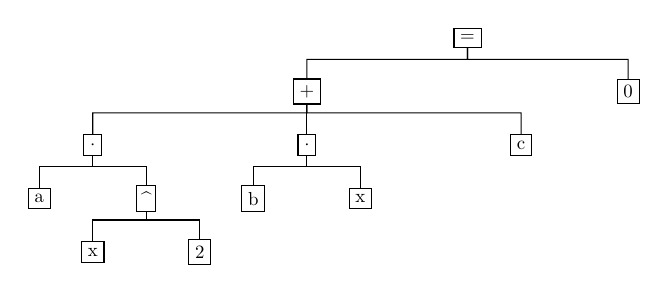
\begin{tikzpicture}[scale=.68, transform shape,
  level 1/.style={sibling distance=4cm,level distance=.8cm}
  ]
  \node[draw] {=}
  [grow via three points={one child at (0,-1.25) and two children at
(-3,-1) and (3,-1)}, edge from parent fork down]
  child {node[draw] {+}[grow via three points={one child at (0,-1) and
two children at (-2,-1) and (2,-1)}, edge from parent fork down]
  child {node[draw] {$\cdot$}[grow via three points={one child at
      (0,-1) and two children at (-1,-1) and (1,-1)}, edge from parent fork down]
    child {node[draw]{a}}
  child {node[draw] {$\,\widehat{}\,$}[grow via three points={one
      child at (0,-1) and two children at (-1,-1) and (1,-1)}, edge from parent fork
    down]
    child {node[draw]{x}}
    child {node[draw]{2}}}
        }
  child {node[draw] {$\cdot$}[grow via three points={one child at
      (0,-1) and two children at (-1,-1) and (1,-1)}, edge from parent fork down]
    child {node[draw]{b}}
    child {node[draw]{x}}
        }
  child {node[draw]{c}}
        }
  child {node[draw] {0}}
  ;
\end{tikzpicture}

\end{minipage}
%\doublespacing

Observe that the transformation tries hard to recognise elided multiplications.
In addition, our procedure contains a number of heuristics, in particular to
\begin{inparaenum}
 \item determine potential function applications,
 \item break up symbol sequences into elided products,
 \item recognise scope and nesting of big operators (e.g., sums, integrals),
 \item distinguish tables into matrices, vectors, and case statements,
 \item combine punctuated expressions and determine the meaning of ellipses.
\end{inparaenum}

Technically the tree is constructed by analysing MathML elements, interpreting
their type, role and font, and turning them into semantic nodes, with parent
pointer and a variable number of children.  In addition we have a notion of
content elements for each node. This is a possibly empty list of semantic nodes
that are combined or abstracted over by this particular node.

For example, a node representing the application of a single operator like $+$,
to a variable number of summands, will have only the semantic nodes representing
the summands as children, while retaining all the intermediate occurrences of
$+$ in its list of content nodes. This allows us to keep a connection between
nodes of the semantic tree and elements in the original MathML structure for
tasks like synchronised highlighting or the semantic enrichment we will discuss
in the next section.


\subsection{Embedding into MathML}
\label{sec:embedding}

The basic idea of embedding the semantic tree into MathML is by modelling the
components of the tree via additional data attributes in the single elements of
the MathML expression. We have decided on data attributes over alternative
means, e.g., exploiting Presentation MathML's semantics tag, RDFa, or micro
data, for a number of reasons: primarily, we want to embed the semantic
structure into the presentation element to provide a different view on the
MathML expression, rather than having a new structure in parallel instead.
Thereby data attributes provide a fast means of retrieving information from the
DOM, which is fully consistent with HTML5 practices.

In practice, we add new data attributes to reflect both content and structure of
the semantic tree. The former are attributes reflecting type, role and font
information stored in each node of the tree. The latter effectively provide each
node with a unique semantic id, and, if necessary, a parent pointer and lists of
pointers to children and content nodes. In addition we have attributes that
provide administrative information with respect to artefacts that have been
introduced or omitted due to the mapping onto the MathML expression.

In the majority of cases the embedding is straight forward, with as little
modification to the original MathML expression as possible. However, this can
not always be maintained for more complex structures. As a consequence we have
the following cases to consider:

\paragraph{Extra Groupings} are often necessary to break up flat rows of
operators and identifiers in order to reflect the term tree structure of the
inferred semantics. These are achieved by grouping elements inside additional
\texttt{mrow} elements to reflect the layers of the term tree.


\paragraph{Added Invisible Elements} are necessary when the semantic
interpretation determines elided operators, such as implicit multiplications or
function applications. Additional \texttt{mo} elements will be introduced containing
unicode characters like invisible times, invisible comma or function
application.

If we consider again the example of the quadratic equation, the enriched
Presentation MathML will look like this:

{\scriptsize\begin{lstlisting}[language=html]
<math type="relseq" role="equality" id="16" children="15,10" content="9">
 <mrow type="infixop" role="addition" id="15" children="12,14,8" content="4,7" parent="16">
  <mrow type="infixop" role="implicit" id="12" children="0,3" content="11" parent="15">
   <mi type="identifier" role="latinletter" id="0" parent="12">a</mi>
   <mo type="operator" role="multiplication" id="11" parent="12" added="true">&#x2062;</mo>
   <msup type="superscript" role="latinletter" id="3" children="1,2" parent="12">
    <mi type="identifier" role="latinletter" id="1" parent="3">x</mi>
    <mn type="number" role="integer" id="2" parent="3">2</mn>
   </msup>
  </mrow>
  <mo type="operator" role="addition" id="4" parent="15">+</mo>
  <mrow type="infixop" role="implicit" id="14" children="5,6" content="13" parent="15">
   <mi type="identifier" role="latinletter" id="5" parent="14">b</mi>
   <mo type="operator" role="multiplication" id="13" parent="14" added="true">&#x2062;</mo>
   <mi type="identifier" role="latinletter" id="6" parent="14">x</mi>
  </mrow>
  <mo type="operator" role="addition" id="7" parent="15">+</mo>
  <mi type="identifier" role="latinletter" id="8" parent="15">c</mi>
 </mrow>
 <mo type="relation" role="equality" id="9" parent="16">=</mo>
 <mn type="number" role="integer" id="10" parent="16">0</mn>
</math>
\end{lstlisting}}
\noindent Observe that the element now contains both extra groupings and
invisible times applications, which are marked as newly added.

\paragraph{Empty Elements} need to be added in case the semantic interpretation
contains mandatory, possibly empty elements, that might not be present in the
presentation. As an example, consider an integral expression consisting of three
parts:
\begin{inparaenum}[(1)]
\item the integration sign, possibly with embellishments like limits,
\item the integrand, and
\item the integral variable.
\end{inparaenum}
If either of the latter two components is not present, they are represented by
an empty element. This is reflected by introducing an empty \texttt{mrow} element in the
Presentation MathML tree, which does not change the visual appearance of the
rendered expression.


\paragraph{Collapsed Elements} can occur when the semantic interpretation
introduces additional structure that can not easily be reflected in the
presentation element without potentially altering the visual rendering. For
example, when semantically indicated, combined sub- and superscript elements
will be represented as subscript with a superscript. This leads to an additional
layer in the tree that is not present in the presentation element, and that can
not be introduced without changing rendering behaviour.  Consequently, the
omitted structure is given in a Lisp-like notation to avoid unconnected pointers
and to ease potential reconstruction of the semantic from the attributes alone.


\paragraph{Special Cases} are complex elements such as \texttt{mfenced} or
\texttt{mmultiscripts}. For example, in the case of the former the semantic
interpretation needs to consider components of the expression that are only
given implicitly via element attributes. In detail, \texttt{mfenced} allows an author to
specify both fences as attributes \texttt{open} and \texttt{close}; absence of
fences is enforced by giving empty string arguments as attribute values, while
omitting the attributes leads to parentheses being inserted as
default. Similarly, a \texttt{separators} attribute allows to specify a list of
characters that should be rendered between children of the \texttt{mfenced} element. For
semantic interpretation these attributes need to be expanded and represented
explicitly in the semantic tree, which in many cases makes it difficult and
sometimes impossible to map the semantic structure back onto the original MathML
element.  Consequently, the original \texttt{mfenced} element is replaced by an explicit
\texttt{mrow}, with opening and closing fences as well as separators modelled 
as proper
new MathML elements. While this might lead to a considerably altered MathML
expression, it is necessary to capture fully semantic meaning, as we observe
with the following example, where the \texttt{separators} attribute is abused to
model operations as well:
\[\{x+y,x,y\}\]

\begin{minipage}{0.2\textwidth}\footnotesize
\begin{lstlisting}[language=html]
<mfenced
 open="{" close="}"
 separators="+,">
  <mi>x</mi>
  <mi>y</mi>
  <mi>x</mi>
  <mi>y</mi>
</mfenced>
\end{lstlisting}
\end{minipage}
\begin{minipage}{0.4\textwidth}
\qquad
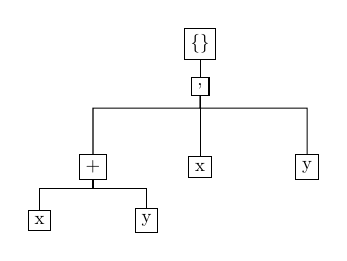
\begin{tikzpicture}[scale=.68, transform shape,
  level 1/.style={sibling distance=2cm,level distance=.8cm}
  ]
  \node[draw] {\{\}}
  child {node[draw] {,}[grow via three points={one child at (0,-.5) and two children at
      (-1,-1) and (1,-1)}, edge from parent fork down]
    child {node[draw] {$+$}
      child {node[draw]{x}}
      child {node[draw]{y}}
    }
    child {node[draw]{x}}
    child {node[draw]{y}}
  }
  ;
\end{tikzpicture}
\end{minipage}

\begin{minipage}{.8\linewidth}\scriptsize
\begin{lstlisting}[language=html]
<mrow type="fenced" role="leftright" id="11" children="10" content="7,8">
 <mo type="fence" role="open" id="7" parent="11" added="true">{</mo>
 <mrow type="punctuated" role="sequence" id="10" children="9,5,2,6,3" content="5,6" parent="11">
  <mrow type="infixop" role="addition" id="9" children="0,1" content="4" parent="10">
   <mi type="identifier" role="latinletter" id="0" parent="9">x</mi>
   <mo type="operator" role="addition" id="4" parent="9" added="true">+</mo>
   <mi type="identifier" role="latinletter" id="1" parent="9">y</mi>
  </mrow>
  <mo type="punctuation" role="comma" id="5" parent="10" added="true">,</mo>
  <mi type="identifier" role="latinletter" id="2" parent="10">x</mi>
  <mo type="punctuation" role="comma" id="6" parent="10" added="true">,</mo>
  <mi type="identifier" role="latinletter" id="3" parent="10">y</mi>
 </mrow>
 <mo type="fence" role="close" id="8" parent="11" added="true">}</mo>
</mrow>
\end{lstlisting}
\end{minipage}

\section{Responsive Equations}
\label{sec:responsive-equations}

Responsive design enhances a core feature of HTML: reflow. Originally focusing
on re-arranging and optimising content, new tools transform the content itself,
e.g., cropping images\cite{web1}, abstracting icons \cite{smashSvg}, or
modifying tables~\cite{zurbTable}.

Reflowing mathematics poses a great challenge as it combines the properties of
text, tables, and graphics into a singular problem. While good line-breaking
algorithms exist for print, they are often counter-productive on the web,
damaging legibility of larger equations beyond repair. The problem is
exacerbated by the fact that content is created with print in mind, manually
fitting it to page dimensions -- manual line breaks, arrangements across tabular
layout, and other \emph{tweaks} prevent a sensible reflow.

We leverage the semantic enrichment to create \emph{responsive equations}, a
completely novel way of dynamically presenting math on small screens. Before
approaching rendering on small screens, a crucial consideration lies in the 
user story for accessing documents with mathematical content on small 
devices in general. In other words, the design has to adapt to the specific use 
case that an author and designer has identified.

Our approach is targeted at what might be called \emph{casual} reading. This 
includes scenarios such as browsing through lists of recent publications 
(e.g.,~repository or journal news feed), cross-reading a publication, and
looking up references. In these use cases, the reader's primary interest does 
not lie in being able to fully access every MathML fragment immediately. 
Rather, in this scenario we need to reduce visual noise to enable 
users to efficiently reach their goal. At the same time, the mathematical 
fragment cannot simply be hidden as it often serves a structural role in the 
overall content and can also be the specific target of the user (e.g., a labelled 
equation). This might be compared to the rendering of maps, though in reverse: 
when a user zooms out, they do not want the map to be cluttered with pointers to 
the most detailed level of information, and yet they need to be able to access 
that level of detail should they need to.


Therefore, our current approach is
\begin{inparaenum}[(a)]
\item to collapse and re-arrange sub-expressions on small screens to provide the
  reader with a meaningful overview of the expression and
\item to implement an interface for exploration of collapsed equations.
\end{inparaenum}
We first discuss the machinery for the exploration and present examples in the
next section.

\subsection{Exploring Equations}
\label{sec:animating}


Since an equation in a collapsed state hides parts of its content, the
responsive rendering mode requires a user interface for exploration.

For the first iteration of this project we have chosen a straight-forward
implementation using MathML's
\texttt{maction} element with \texttt{actiontype} set to \texttt{toggle}, cf. 
\cite[3.7.1]{MML}. This will
allow users to explore the content using click, keyboard, and touch events.
The \texttt{maction} elements are nested so that only the next level of the
collapse is revealed.

The element indicating collapsed content is currently a simple Unicode 
construction, \collapse{X}, with X indicating the top-level structure that was 
collapsed. Currently, we differentiate the following structures:

\noindent\begin{minipage}[t]{.34\linewidth}
  \begin{itemize}
  \item Matched fences: \collapse{[)} etc.
  \item Function application: \collapse{f()}
  \item Fraction: \collapse{/}
  \item Surds: \collapse{\raise2pt\hbox{$\sqrt{}$}\,}
  \item Scripts: \collapse{\lower1pt\hbox{$\square$}\raise1.2ex\hbox{.}},
    \collapse{\lower1pt\hbox{$\square$}\text{.}},
    \collapse{\lower1pt\hbox{$\square$}\text{:}}
  \item Large operators: \collapse{\mathrm{\Sigma}} etc.
  \end{itemize}
\end{minipage}
\begin{minipage}[t]{.34\linewidth}
  \begin{itemize}
  \item Repeated operators: \collapse{+} etc.
  \item Long identifier: \collapse{\text{x}}
  \item Long number: \collapse{\#}
  \item Long text: \collapse{\ldots}
  \item Vector: \collapse{\langle:\rangle}
  \item Square Matrix: \collapse{[::]}
  \end{itemize}
\end{minipage}
\begin{minipage}[t]{.32\linewidth}
  \begin{itemize}
  \item Row vector: \collapse{\langle\cdots\rangle}
  \item Column vector:
    \collapse{\langle\smash{\lower2pt\hbox{$\vdots$}}\rangle}▶
  \item Unknown matrix: \collapse{(::)}
  \item Punctuated text: \collapse{...}
  \item Punctuated gen.: \collapse{,} etc.
  \end{itemize}
\end{minipage}\vspace{1ex}

Although currently fixed, authors will be able to customise these placeholders
in the future, using Unicode, CSS, or SVG.

While \texttt{maction toggles} are simple and standard, the user 
experience is not ideal. For example, it is too easy to accidentally 
trigger a collapse of parts of the equation. Similarly, it is difficult to 
quickly un-collapse the entire equations. As we gain experience, we hope to be 
able to augment the regular toggle and feed that experience back into the 
development of the MathML specification.

\subsection{Complexity Measure}
\label{sec:complexity}

Since collapsing is intended to shorten an expression when space is at
a premium, one approach to determining what to collapse would be
based on the widths of the various terms.  For our algorithm,
however, the widths of the terms are not yet known (as the widths are
not computed until the terms are typeset for output, while the potential
collapses are determined before the output process begins).  Instead
of width, our approach is to use a measure of complexity of the terms
as a surrogate for width.  (As a side-effect, this makes it possible
to collapse for reasons other than saving space -- see the section on
size versus content in section \ref{sec:discussion} below.)

Each term in the MathML expression is assigned a complexity value
based on the length of its content or the complexity of its children.
A MathML token element (like an identifier or a number) is given a
complexity determined by the number of characters in the text of
the element; a longer identifier or number has a higher complexity
(since we want complexity to act as a replacement for width).  Other
elements, like square roots, or fractions, have their complexity
determined by combining the complexity of their child nodes.

For example, an expression that consists of a combination of three
terms will have a complexity that is the sum of the complexities of
the individual terms and the complexities of the operators that joins
them.  Because we want combinations that involve more terms to be more
likely to collapse than those with few terms, the complexity is
augmented by a factor based on the number of children (regardless of
the complexities of the individual terms).  So in the sum $a+b$,
suppose the $a$, $+$, and $b$ are each assigned a complexity of 1,
then the complexity of the sum might be 6 (3 for the sum of the
complexities of the element of the sum, and 3 more for the fact that
there are three children of the expression).

In a similar fashion, a fraction might have complexity that is the
sum of the complexities of the numerator and denominator, plus an
additional amount for being a fraction, while a square root's
complexity might be the complexity of its argument plus something
more for being a square root.

In this way, each term in the MathML tree is given a complexity.
This value is used to decide whether the term should be collapsible
or not.  The cut-off value that determines this is based on the
semantic type of the MathML element.  For example, if the cut-off
value for a sum was set to 12, then the sum $a+b+c$ (with a complexity
of 10) would not be collapsible, while $a+b+c+d$ (with a complexity of
14) would be, and $100+100+100$ (with a complexity of 14.5) would
also be collapsible.

All the parameters involved in the complexity computations (e.g., the
weight of each character in a token element, the weights of child
terms, the extra amount for a fraction or root, and the cut-off values
for collapsing) are stored in tables that can be adjusted by the
page author, should the default settings not provide suitable
collapses for the equations in use on the page.


\section{Examples and Initial Results}
\label{sec:results}

For development and experimentation we avoid manual doctoring of examples, but
look for examples ``in the wild''; this aligns with our focus on handling
arbitrary content well, not on handling well-prepared content excellently.  We
therefore give an overview of the core features and challenges of our approach,
by further exploring the example from the introduction that we have found on
\href{http://math.stackexchange.com/a/1285149}{math.stackexchange.com} as the
following original {\LaTeX} code:


{\tiny
\begin{lstlisting}[language=TeX]
\begin{align}
I_\nu(\nu^{-1},1)
&=\underbrace{\frac{\pi^2}{4}\ln\left(\frac{(1+\nu)^{1+\nu}}{\nu^\nu}
\right)-\frac{7\zeta(3)}{8}\nu}_{\text{Let this be 
C}}+2\int^\frac{1-\nu}{1+\nu}_1\frac{\chi_3(v)}{(1+v)^2}{\rm d}v\\
&=C-\left.\frac{2\chi_3(v)}{1+v}\right|^\frac{1-\nu}{1+\nu}_1+2\int^\frac{1-\nu}
{1+\nu}_1\frac{\chi_2(v)}{v(1+v)}{\rm d}v\\
&=C+(1-\nu)\chi_3\left(\frac{1-\nu}{1+\nu}\right)-\frac{7\zeta(3)}{8}
-\left.\color{white}{\frac{1}{1}}2\chi_2(v)\ln(1+v)\right|^\frac{1-\nu}{1+\nu}
_1+\int^\frac{1-\nu}{1+\nu}_1\frac{\ln(1+v)\ln\left(\frac{1+v}{1-v}\right)}{v}{
\rm d}v\\
&=C+(1-\nu)\chi_3\left(\frac{1-\nu}{1+\nu}\right)-\frac{7\zeta(3)}{8}
+2\chi_2\left(\frac{1-\nu}{1+\nu}\right)\ln\left(\frac{1+\nu}{2}\right)+\frac{
\pi^2}{4}\ln{2}\\
&\ \ \ \ 
+\frac{1}{2}\int^\frac{1-\nu}{1+\nu}_1\frac{
\ln^2(1+v)-\ln^2(1-v)+\ln^2\left(\frac{1-v}{1+v}\right)}{v}{\rm d}v
\end{align}
\end{lstlisting}
} Note that the source contains a few artefacts such as an \emph{invisible} (in
fact, white) fraction as well as manual spacing.

% <math xmlns="http://www.w3.org/1998/Math/MathML" display="block">
%   <mtable columnalign="right left right left right left right left right left 
% right left" rowspacing="3pt" columnspacing="0em 2em 0em 2em 0em 2em 0em 2em 0em 
% 2em 0em" displaystyle="true">
%     <mtr>
%       <mtd>
%         <msub>
%           <mi>I</mi>
%           <mi mathvariant="italic">&#x03BD;<!-- ν --></mi>
%         </msub>
%         <mo stretchy="false">(</mo>
%         <msup>
%           <mi mathvariant="italic">&#x03BD;<!-- ν --></mi>
%           <mrow class="MJX-TeXAtom-ORD">
%             <mo>&#x2212;<!-- − --></mo>
%             <mn>1</mn>
%           </mrow>
%         </msup>
%         <mo>,</mo>
%         <mn>1</mn>
%         <mo stretchy="false">)</mo>
%       </mtd>
%       <mtd>
%         <mi></mi>
%         <mo>=</mo>
%         <munder>
%           <mrow class="MJX-TeXAtom-OP">
%             <munder>
%               <mrow>
%                 <mfrac>
%                   <msup>
%                     <mi mathvariant="italic">&#x03C0;<!-- π --></mi>
%                     <mn>2</mn>
%                   </msup>
%                   <mn>4</mn>
%                 </mfrac>
%                 <mi>ln</mi>
%                 <mrow>
%                   <mo fence="true">(</mo>
%                   <mfrac>
%                     <mrow>
%                       <mo stretchy="false">(</mo>
%                       <mn>1</mn>
%                       <mo>+</mo>
%                       <mi mathvariant="italic">&#x03BD;<!-- ν --></mi>
%                       <msup>
%                         <mo stretchy="false">)</mo>
%                         <mrow class="MJX-TeXAtom-ORD">
%                           <mn>1</mn>
%                           <mo>+</mo>
%                           <mi mathvariant="italic">&#x03BD;<!-- ν --></mi>
%                         </mrow>
%                       </msup>
%                     </mrow>
%                     <msup>
%                       <mi mathvariant="italic">&#x03BD;<!-- ν --></mi>
%                       <mi mathvariant="italic">&#x03BD;<!-- ν --></mi>
%                     </msup>
%                   </mfrac>
%                   <mo fence="true">)</mo>
%                 </mrow>
%                 <mo>&#x2212;<!-- − --></mo>
%                 <mfrac>
%                   <mrow>
%                     <mn>7</mn>
%                     <mi mathvariant="italic">&#x03B6;<!-- ζ --></mi>
%                     <mo stretchy="false">(</mo>
%                     <mn>3</mn>
%                     <mo stretchy="false">)</mo>
%                   </mrow>
%                   <mn>8</mn>
%                 </mfrac>
%                 <mi mathvariant="italic">&#x03BD;<!-- ν --></mi>
%               </mrow>
%               <mo accent="true">&#x23DF;<!-- ⏟ --></mo>
%             </munder>
%           </mrow>
%           <mrow class="MJX-TeXAtom-ORD">
%             <mtext>Let this be 
% C</mtext>
%           </mrow>
%         </munder>
%         <mo>+</mo>
%         <mn>2</mn>
%         <msubsup>
%           <mo>&#x222B;<!-- ∫ --></mo>
%           <mn>1</mn>
%           <mfrac>
%             <mrow>
%               <mn>1</mn>
%               <mo>&#x2212;<!-- − --></mo>
%               <mi mathvariant="italic">&#x03BD;<!-- ν --></mi>
%             </mrow>
%             <mrow>
%               <mn>1</mn>
%               <mo>+</mo>
%               <mi mathvariant="italic">&#x03BD;<!-- ν --></mi>
%             </mrow>
%           </mfrac>
%         </msubsup>
%         <mfrac>
%           <mrow>
%             <msub>
%               <mi mathvariant="italic">&#x03C7;<!-- χ --></mi>
%               <mn>3</mn>
%             </msub>
%             <mo stretchy="false">(</mo>
%             <mi>v</mi>
%             <mo stretchy="false">)</mo>
%           </mrow>
%           <mrow>
%             <mo stretchy="false">(</mo>
%             <mn>1</mn>
%             <mo>+</mo>
%             <mi>v</mi>
%             <msup>
%               <mo stretchy="false">)</mo>
%               <mn>2</mn>
%             </msup>
%           </mrow>
%         </mfrac>
%         <mrow class="MJX-TeXAtom-ORD">
%           <mi mathvariant="normal">d</mi>
%         </mrow>
%         <mi>v</mi>
%       </mtd>
%     </mtr>
%     <mtr>
%       <mtd />
%       <mtd>
%         <mi></mi>
%         <mo>=</mo>
%         <mi>C</mi>
%         <mo>&#x2212;<!-- − --></mo>
%         <msubsup>
%           <mrow>
%             <mo fence="true" stretchy="true"></mo>
%             <mfrac>
%               <mrow>
%                 <mn>2</mn>
%                 <msub>
%                   <mi mathvariant="italic">&#x03C7;<!-- χ --></mi>
%                   <mn>3</mn>
%                 </msub>
%                 <mo stretchy="false">(</mo>
%                 <mi>v</mi>
%                 <mo stretchy="false">)</mo>
%               </mrow>
%               <mrow>
%                 <mn>1</mn>
%                 <mo>+</mo>
%                 <mi>v</mi>
%               </mrow>
%             </mfrac>
%             <mo fence="true">|</mo>
%           </mrow>
%           <mn>1</mn>
%           <mfrac>
%             <mrow>
%               <mn>1</mn>
%               <mo>&#x2212;<!-- − --></mo>
%               <mi mathvariant="italic">&#x03BD;<!-- ν --></mi>
%             </mrow>
%             <mrow>
%               <mn>1</mn>
%               <mo>+</mo>
%               <mi mathvariant="italic">&#x03BD;<!-- ν --></mi>
%             </mrow>
%           </mfrac>
%         </msubsup>
%         <mo>+</mo>
%         <mn>2</mn>
%         <msubsup>
%           <mo>&#x222B;<!-- ∫ --></mo>
%           <mn>1</mn>
%           <mfrac>
%             <mrow>
%               <mn>1</mn>
%               <mo>&#x2212;<!-- − --></mo>
%               <mi mathvariant="italic">&#x03BD;<!-- ν --></mi>
%             </mrow>
%             <mrow>
%               <mn>1</mn>
%               <mo>+</mo>
%               <mi mathvariant="italic">&#x03BD;<!-- ν --></mi>
%             </mrow>
%           </mfrac>
%         </msubsup>
%         <mfrac>
%           <mrow>
%             <msub>
%               <mi mathvariant="italic">&#x03C7;<!-- χ --></mi>
%               <mn>2</mn>
%             </msub>
%             <mo stretchy="false">(</mo>
%             <mi>v</mi>
%             <mo stretchy="false">)</mo>
%           </mrow>
%           <mrow>
%             <mi>v</mi>
%             <mo stretchy="false">(</mo>
%             <mn>1</mn>
%             <mo>+</mo>
%             <mi>v</mi>
%             <mo stretchy="false">)</mo>
%           </mrow>
%         </mfrac>
%         <mrow class="MJX-TeXAtom-ORD">
%           <mi mathvariant="normal">d</mi>
%         </mrow>
%         <mi>v</mi>
%       </mtd>
%     </mtr>
%     <mtr>
%       <mtd />
%       <mtd>
%         <mi></mi>
%         <mo>=</mo>
%         <mi>C</mi>
%         <mo>+</mo>
%         <mo stretchy="false">(</mo>
%         <mn>1</mn>
%         <mo>&#x2212;<!-- − --></mo>
%         <mi mathvariant="italic">&#x03BD;<!-- ν --></mi>
%         <mo stretchy="false">)</mo>
%         <msub>
%           <mi mathvariant="italic">&#x03C7;<!-- χ --></mi>
%           <mn>3</mn>
%         </msub>
%         <mrow>
%           <mo fence="true">(</mo>
%           <mfrac>
%             <mrow>
%               <mn>1</mn>
%               <mo>&#x2212;<!-- − --></mo>
%               <mi mathvariant="italic">&#x03BD;<!-- ν --></mi>
%             </mrow>
%             <mrow>
%               <mn>1</mn>
%               <mo>+</mo>
%               <mi mathvariant="italic">&#x03BD;<!-- ν --></mi>
%             </mrow>
%           </mfrac>
%           <mo fence="true">)</mo>
%         </mrow>
%         <mo>&#x2212;<!-- − --></mo>
%         <mfrac>
%           <mrow>
%             <mn>7</mn>
%             <mi mathvariant="italic">&#x03B6;<!-- ζ --></mi>
%             <mo stretchy="false">(</mo>
%             <mn>3</mn>
%             <mo stretchy="false">)</mo>
%           </mrow>
%           <mn>8</mn>
%         </mfrac>
%         <mo>&#x2212;<!-- − --></mo>
%         <msubsup>
%           <mrow>
%             <mo fence="true" stretchy="true"></mo>
%             <mstyle mathcolor="white">
%               <mfrac>
%                 <mn>1</mn>
%                 <mn>1</mn>
%               </mfrac>
%             </mstyle>
%             <mn>2</mn>
%             <msub>
%               <mi mathvariant="italic">&#x03C7;<!-- χ --></mi>
%               <mn>2</mn>
%             </msub>
%             <mo stretchy="false">(</mo>
%             <mi>v</mi>
%             <mo stretchy="false">)</mo>
%             <mi>ln</mi>
%             <mo>&#x2061;<!-- ⁡ --></mo>
%             <mo stretchy="false">(</mo>
%             <mn>1</mn>
%             <mo>+</mo>
%             <mi>v</mi>
%             <mo stretchy="false">)</mo>
%             <mo fence="true">|</mo>
%           </mrow>
%           <mn>1</mn>
%           <mfrac>
%             <mrow>
%               <mn>1</mn>
%               <mo>&#x2212;<!-- − --></mo>
%               <mi mathvariant="italic">&#x03BD;<!-- ν --></mi>
%             </mrow>
%             <mrow>
%               <mn>1</mn>
%               <mo>+</mo>
%               <mi mathvariant="italic">&#x03BD;<!-- ν --></mi>
%             </mrow>
%           </mfrac>
%         </msubsup>
%         <mo>+</mo>
%         <msubsup>
%           <mo>&#x222B;<!-- ∫ --></mo>
%           <mn>1</mn>
%           <mfrac>
%             <mrow>
%               <mn>1</mn>
%               <mo>&#x2212;<!-- − --></mo>
%               <mi mathvariant="italic">&#x03BD;<!-- ν --></mi>
%             </mrow>
%             <mrow>
%               <mn>1</mn>
%               <mo>+</mo>
%               <mi mathvariant="italic">&#x03BD;<!-- ν --></mi>
%             </mrow>
%           </mfrac>
%         </msubsup>
%         <mfrac>
%           <mrow>
%             <mi>ln</mi>
%             <mo>&#x2061;<!-- ⁡ --></mo>
%             <mo stretchy="false">(</mo>
%             <mn>1</mn>
%             <mo>+</mo>
%             <mi>v</mi>
%             <mo stretchy="false">)</mo>
%             <mi>ln</mi>
%             <mrow>
%               <mo fence="true">(</mo>
%               <mfrac>
%                 <mrow>
%                   <mn>1</mn>
%                   <mo>+</mo>
%                   <mi>v</mi>
%                 </mrow>
%                 <mrow>
%                   <mn>1</mn>
%                   <mo>&#x2212;<!-- − --></mo>
%                   <mi>v</mi>
%                 </mrow>
%               </mfrac>
%               <mo fence="true">)</mo>
%             </mrow>
%           </mrow>
%           <mi>v</mi>
%         </mfrac>
%         <mrow class="MJX-TeXAtom-ORD">
%           <mi mathvariant="normal">d</mi>
%         </mrow>
%         <mi>v</mi>
%       </mtd>
%     </mtr>
%     <mtr>
%       <mtd />
%       <mtd>
%         <mi></mi>
%         <mo>=</mo>
%         <mi>C</mi>
%         <mo>+</mo>
%         <mo stretchy="false">(</mo>
%         <mn>1</mn>
%         <mo>&#x2212;<!-- − --></mo>
%         <mi mathvariant="italic">&#x03BD;<!-- ν --></mi>
%         <mo stretchy="false">)</mo>
%         <msub>
%           <mi mathvariant="italic">&#x03C7;<!-- χ --></mi>
%           <mn>3</mn>
%         </msub>
%         <mrow>
%           <mo fence="true">(</mo>
%           <mfrac>
%             <mrow>
%               <mn>1</mn>
%               <mo>&#x2212;<!-- − --></mo>
%               <mi mathvariant="italic">&#x03BD;<!-- ν --></mi>
%             </mrow>
%             <mrow>
%               <mn>1</mn>
%               <mo>+</mo>
%               <mi mathvariant="italic">&#x03BD;<!-- ν --></mi>
%             </mrow>
%           </mfrac>
%           <mo fence="true">)</mo>
%         </mrow>
%         <mo>&#x2212;<!-- − --></mo>
%         <mfrac>
%           <mrow>
%             <mn>7</mn>
%             <mi mathvariant="italic">&#x03B6;<!-- ζ --></mi>
%             <mo stretchy="false">(</mo>
%             <mn>3</mn>
%             <mo stretchy="false">)</mo>
%           </mrow>
%           <mn>8</mn>
%         </mfrac>
%         <mo>+</mo>
%         <mn>2</mn>
%         <msub>
%           <mi mathvariant="italic">&#x03C7;<!-- χ --></mi>
%           <mn>2</mn>
%         </msub>
%         <mrow>
%           <mo fence="true">(</mo>
%           <mfrac>
%             <mrow>
%               <mn>1</mn>
%               <mo>&#x2212;<!-- − --></mo>
%               <mi mathvariant="italic">&#x03BD;<!-- ν --></mi>
%             </mrow>
%             <mrow>
%               <mn>1</mn>
%               <mo>+</mo>
%               <mi mathvariant="italic">&#x03BD;<!-- ν --></mi>
%             </mrow>
%           </mfrac>
%           <mo fence="true">)</mo>
%         </mrow>
%         <mi>ln</mi>
%         <mrow>
%           <mo fence="true">(</mo>
%           <mfrac>
%             <mrow>
%               <mn>1</mn>
%               <mo>+</mo>
%               <mi mathvariant="italic">&#x03BD;<!-- ν --></mi>
%             </mrow>
%             <mn>2</mn>
%           </mfrac>
%           <mo fence="true">)</mo>
%         </mrow>
%         <mo>+</mo>
%         <mfrac>
%           <msup>
%             <mi mathvariant="italic">&#x03C0;<!-- π --></mi>
%             <mn>2</mn>
%           </msup>
%           <mn>4</mn>
%         </mfrac>
%         <mi>ln</mi>
%         <mrow class="MJX-TeXAtom-ORD">
%           <mn>2</mn>
%         </mrow>
%       </mtd>
%     </mtr>
%     <mtr>
%       <mtd />
%       <mtd>
%         <mtext>&#xA0;</mtext>
%         <mtext>&#xA0;</mtext>
%         <mtext>&#xA0;</mtext>
%         <mtext>&#xA0;</mtext>
%         <mo>+</mo>
%         <mfrac>
%           <mn>1</mn>
%           <mn>2</mn>
%         </mfrac>
%         <msubsup>
%           <mo>&#x222B;<!-- ∫ --></mo>
%           <mn>1</mn>
%           <mfrac>
%             <mrow>
%               <mn>1</mn>
%               <mo>&#x2212;<!-- − --></mo>
%               <mi mathvariant="italic">&#x03BD;<!-- ν --></mi>
%             </mrow>
%             <mrow>
%               <mn>1</mn>
%               <mo>+</mo>
%               <mi mathvariant="italic">&#x03BD;<!-- ν --></mi>
%             </mrow>
%           </mfrac>
%         </msubsup>
%         <mfrac>
%           <mrow>
%             <msup>
%               <mi>ln</mi>
%               <mn>2</mn>
%             </msup>
%             <mo>&#x2061;<!-- ⁡ --></mo>
%             <mo stretchy="false">(</mo>
%             <mn>1</mn>
%             <mo>+</mo>
%             <mi>v</mi>
%             <mo stretchy="false">)</mo>
%             <mo>&#x2212;<!-- − --></mo>
%             <msup>
%               <mi>ln</mi>
%               <mn>2</mn>
%             </msup>
%             <mo>&#x2061;<!-- ⁡ --></mo>
%             <mo stretchy="false">(</mo>
%             <mn>1</mn>
%             <mo>&#x2212;<!-- − --></mo>
%             <mi>v</mi>
%             <mo stretchy="false">)</mo>
%             <mo>+</mo>
%             <msup>
%               <mi>ln</mi>
%               <mn>2</mn>
%             </msup>
%             <mrow>
%               <mo fence="true">(</mo>
%               <mfrac>
%                 <mrow>
%                   <mn>1</mn>
%                   <mo>&#x2212;<!-- − --></mo>
%                   <mi>v</mi>
%                 </mrow>
%                 <mrow>
%                   <mn>1</mn>
%                   <mo>+</mo>
%                   <mi>v</mi>
%                 </mrow>
%               </mfrac>
%               <mo fence="true">)</mo>
%             </mrow>
%           </mrow>
%           <mi>v</mi>
%         </mfrac>
%         <mrow class="MJX-TeXAtom-ORD">
%           <mi mathvariant="normal">d</mi>
%         </mrow>
%         <mi>v</mi>
%       </mtd>
%     </mtr>
%   </mtable>
% </math>

To provide a real-world experience, we have simulated a Nexus 5 device using 
the developer tools of the Chrome browsers, with a simulated display size of 
$360\mathrm{px} \times 640\mathrm{px}$. In our sample HTML page, the font size for the 
mathematical fragment is $\mathbin{\sim} 18.5\mathrm{px}$.\footnote{The precise font 
size is determined on the fly to match ex-heights with the surrounding font, 
which may differ across devices.} 


\subsection{Line-breaking}
\begin{wrapfigure}{r}{0.5\textwidth}
  \vspace{-50pt}
  \centering 
  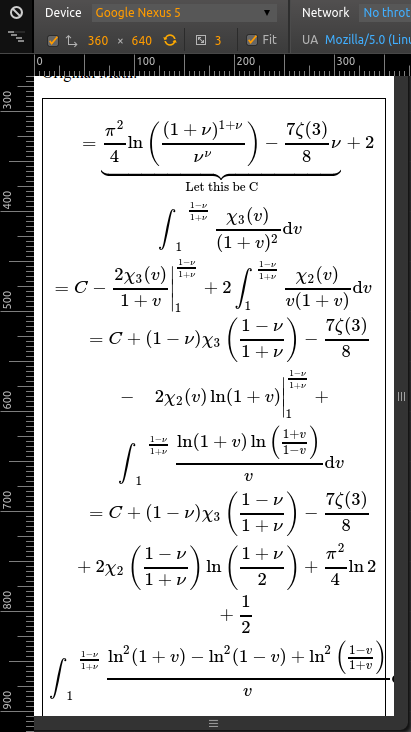
\includegraphics[width=0.49\textwidth]{./ex_long_linebreaking.png}
  \caption{Screenshot: linebreaking\label{ex_long_linebreaking}}
  \vspace{-40pt}
\end{wrapfigure}

Applying line-breaking programmatically to this kind of equation is 
challenging. Align environments have to be interpreted as \texttt{mtable} 
elements as they might have equation labels attached to them which can only 
be implemented inside \texttt{mtable} structures. 
Line-breaking does not touch the table structure and can only perform 
line-breaks within tables. The results are often visually complicated.


In \autoref{ex_long_linebreaking} we see the result of rendering with 
line-breaking\footnote{MathJax implements most of the MathML specification 
regarding line-breaking.} (no enrichment applied)  on an simulated 
smart-phone device. The first observation is that the initial column takes up 
most of the screen already, pushing the second column outside the viewport. In 
other words, line-breaking fails fundamentally to fit the content on the screen, 
just as with other table structures.

For the screenshot we simulated a swipe to bring the second column into
view. Here we encounter additional problems. Since line-breaking occurs within
each cell, there is no way to align the breaks across rows. Instead, iterated
line-breaks in different cells produce an uneven rendering. In addition, we see
how the quality of the markup negatively affects the layout, e.g., in the top
row the linebreak splits a product that forms a single summand. In short, the
result is very difficult to process for the reader. See also
\autoref{sec:improve-default} for further discussion of line-breaking.

\subsection{Collapsing}
\label{sec:collapsing}

  In comparison, the (maximally collapsed) responsive rendering of the equation
  will look like the following.
\begin{align*}
 \collapse{\mathrm{f}()} & = \collapse{+} \\
 & =  \collapse{+} \\ 
 & = \collapse{+} \\ 
 & = \collapse{+} + \collapse{\cdot} + \collapse{\cdot} \\
 & \collapse{...} 
\end{align*}

With a width of 
$\mathbin{\sim} 258\mathrm{px}$, this rendering fits well even on very small 
screens and avoids additional noise. While it collapses the details, it does so 
gracefully, retaining the fundamental layout. 

Since the screen size of the simulated Nexus 5 device is actually larger, our 
current implementation will automatically expand sub-expressions to expose as 
much detail as possible as seen in \autoref{ex_long_collapse}.


\begin{wrapfigure}{r}{0.5\textwidth}
  \vspace{-20pt}
 \centering 
 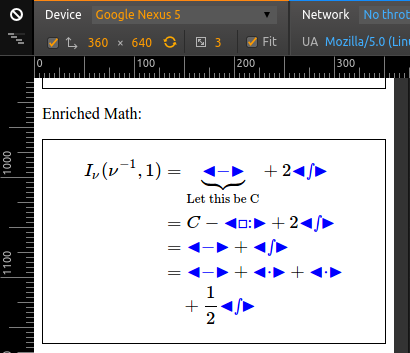
\includegraphics[width=0.49\textwidth]{./ex_long_collapse.png}
 \caption{Screenshot: responsive rendering
\label{ex_long_collapse}}
  \vspace{-20pt}
\end{wrapfigure}

As described earlier, our current implementation uses standard \texttt{maction} 
elements to enable the user to explore the equation. Each placeholder serves as 
a toggle, expanding nested layers of the equation. To provide a final example, 
a reader might then want to explore particular aspects of the expression, 
such as the evolution of the integral term; a sample exploration is captured in
\autoref{ex_long_collapse2}.


\begin{wrapfigure}{r}{0.5\textwidth}
  \vspace{-35pt}
 \centering 
 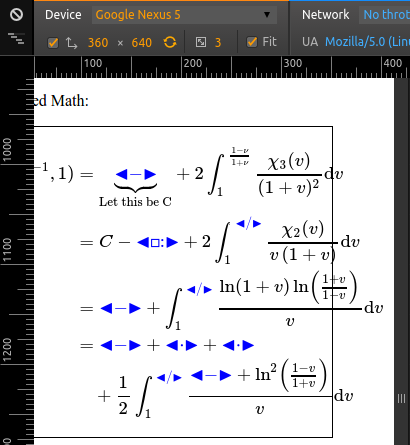
\includegraphics[width=0.49\textwidth]{./ex_long_collapse2.png}
 \caption{Screenshot: exploring responsive rendering
\label{ex_long_collapse2}}
  \vspace{-20pt}
\end{wrapfigure}

As can be seen, the user interface for exploration is still in its infancy and 
we do not, in fact, expect to come up with a smooth implementation. From 
personal experience, this rendering changes the `reading of' (or interaction 
with) an expression significantly and only real user feedback will determine 
which aspects need to be modified.

% 
%  
% \subsection{Comparison with linebreaking}
% \label{sec:linebreaking}
% 
% Consider the following example, a slightly modified version of \cite[equation 
% 3.13]{2015arXiv150504830G}, which in turn was arbitrarily picked from the 
% arXiv. 
% 
% \begin{gather*}
% \geq
% \int\left\langle \Psi_{z},\ \Psi_{z}\right\rangle 
% _{\mbox{E}}\times\left((1-\epsilon)\frac{\left\langle \Psi_{z},\ 
% p^{2}\Psi_{z}\right\rangle _{\mbox{E}}}{\left\langle \Psi_{z},\ 
% \Psi_{z}\right\rangle _{\mbox{E}}}-\frac{\alpha 
% P}{(1-\delta)}\underset{B_{n}}{\sum}\frac{\left|\left\langle \Psi_{z},\ 
% e^{-i\mathbf{\mathcal{K}_{B_{n}}}x}\Psi_{z}\right\rangle 
% _{\mbox{E}}\right|^{2}}{\left|\left\langle \Psi_{z},\ \Psi_{z}\right\rangle 
% _{\mbox{E}}\right|^{2}} + \right.\\
% \left.-\alpha^{2}\frac{\left\langle \Psi_{z},\ V(\alpha 
% x)\Psi_{z}\right\rangle 
% _{\mbox{E}}}{\left\langle \Psi_{z},\ \Psi_{z}\right\rangle 
% _{\mbox{E}}}\right)\prod_{B_{m}}dz_{B_{m}}d\overline{z_{B_{m}}}-(1-\delta)\frac{
% 2K}{P} 
% \end{gather*}
% 
% We have manually added a line break to fit the dimensions of a 
% print page but let us now consider this equation as if on a single line.
% 
% \begin{wrapfigure}{r}{0.5\textwidth}
%  \centering 
%  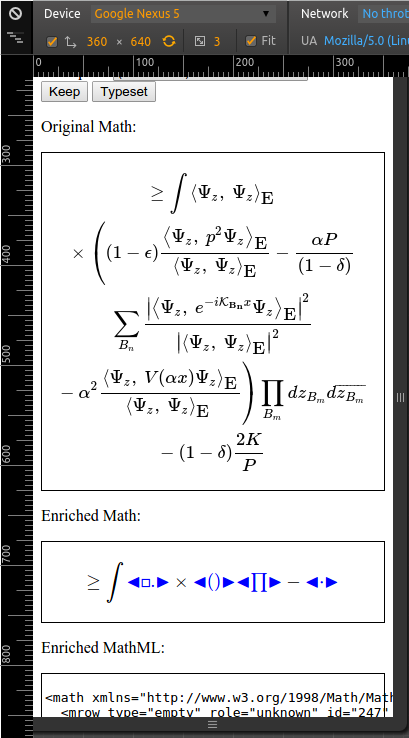
\includegraphics[width=0.49\textwidth]{./ex_breakvsresp.png}
%  \caption{Screenshot: linebreaking vs responsive rendering \label{breakvsresp}}
% \end{wrapfigure}
% 
% In \autoref{breakvsresp}, we include a screenshot capturing a 
% simple website providing a rendering of both line-breaking and responsive 
% rendering. The developer tools of the Chrome browser were used to specify the 
% dimensions of a Nexus 5 smartphone screen. Comparing MathJax's line-breaking 
% alogrithm (which implements most of the MathML specification regarding 
% line-breaking) and the new responsive equation rendering, one can see how the 
% multiple line breaks deteriorate the rendering. The responsive rendering is able 
% to communicate the basic structure of the equation

\subsection{Improving default rendering}
\label{sec:improve-default}

A significant problem in professional publishing 
workflows lies in the low quality of Presentation MathML markup. MathML 
fragments are often produced by third-party vendors who convert documents 
into XML. MathML fragments are either generated from other input 
formats such as TeX/LaTeX code or manually recreated from other renderings
(image, pdf). 
In the latter case, it is unrealistic to expect such conversion 
specialists to have enough domain specific knowledge to capture 
nuances in the semantics and presentation of the mathematical fragments. Even 
in the case of a converter being used, the source markup is often of low 
quality, e.g., TeX lacking appropriate \texttt{\textbackslash right 
\textbackslash left}). This leads to very \emph{flat} MathML fragments. 
Ultimately, the results of this process are too often of poor quality.

The enriched Presentation MathML can resolve some of these issues and 
thus improve rendering in general. This is due to gently enhancing the MathML 
structure, e.g., with missing mrows, matched fences, and so on. 
% <math display="block" xmlns="http://www.w3.org/1998/Math/MathML">
%     <mo stretchy="true">|</mo>
%     <mrow>
%       <msub>
%         <mrow>
%           <mi>τ</mi>
%         </mrow>
%         <mrow>
%           <mn>0</mn>
%         </mrow>
%       </msub>
%     </mrow>
%     <mo stretchy="true">|</mo>
%     <mo>=</mo>
%     <mo stretchy="true">|</mo>
%     <mrow>
%       <munder>
%         <mrow>
%           <mo>∑</mo>
%         </mrow>
%         <mrow>
%           <mi>m</mi>
%         </mrow>
%       </munder>
%       <msub>
%         <mrow>
%           <mi mathvariant="bold">E</mi>
%         </mrow>
%         <mrow>
%           <mn>0</mn>
%           <mi>m</mi>
%         </mrow>
%       </msub>
%       <mo stretchy="true">(</mo>
%       <mrow>
%         <msub>
%           <mrow>
%             <mi>a</mi>
%           </mrow>
%           <mrow>
%             <mi>m</mi>
%           </mrow>
%         </msub>
%         <mo>+</mo>
%         <msub>
%           <mrow>
%             <mi>b</mi>
%           </mrow>
%           <mrow>
%             <mi>m</mi>
%           </mrow>
%         </msub>
%       </mrow>
%       <mo stretchy="true">)</mo>
%     </mrow>
%     <mo stretchy="true">|</mo>
% </math>


The following example reconstructs the first few terms of \cite[Eq. 
17]{Chang-Hasnain:12}.

\[ 
\biggl\vert \tau_0 \biggr\vert = \biggl\vert  \sum_{m} \bigg(a_b + b_m\bigg) 
\bigg\vert 
\]

The reason for these oversized fences lies in the \emph{flat} structure of the 
underlying  Presentation MathML. MathML specifies that 
stretchy fences should match the height of the tallest sub-expression within an 
\texttt{mrow}. The lack of any grouping in the MathML source forces renderers 
to have all fences match the size of the $\sum$. 


\begin{wrapfigure}{r}{0.5\textwidth}
  \vspace{-25pt}
 \centering 
 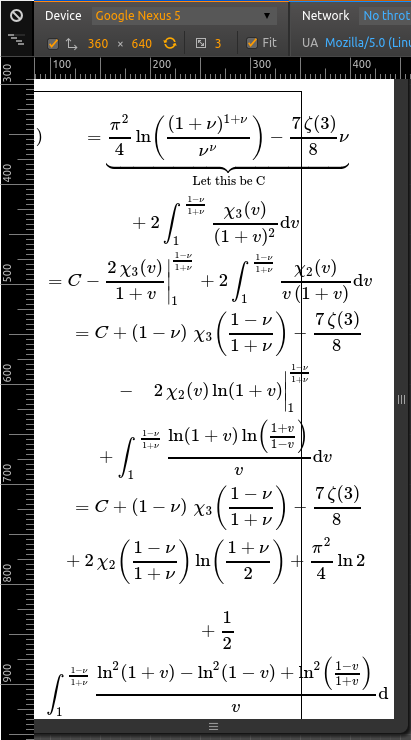
\includegraphics[width=0.49\textwidth]{./ex_long_linebreaking_enriched.png}
 \caption{Screenshot: linebreaking without enrichment \label{break-enrich}}
  \vspace{-45pt}
\end{wrapfigure}

After enriching the MathML, matching fences are identified and 
additional \texttt{mrow}s introduced, leading to improved rendering equivalent 
to the following.

\[ 
\left\vert  \tau_0 \right\vert = \left \vert \sum_{m} \left(a_b + b_m\right) 
\right\vert 
\]

As this may seem like a mild effect we can only stress how 
wide-spread and persistent such problems are in published MathML.

Additionally, these subtle improvements to the markup make it easier for 
line-breaking algorithms to determine good breakpoints. To revisit our 
example, \autoref{break-enrich} consists of a screenshot with line-breaking 
after semantic enrichment. Note how the second line of the first cell and the 
third line of the third cell have improved by grouping the multiplication as 
well as addition correctly.


Anecdotal evidence from sharing our work with other researchers suggests this 
rendering could have the unexpected side effect to alert authors to bad 
practices in their markup. That is, researchers responded to the new rendering 
by stating that they want to author in a way  that renders well responsively. 
While clearly biased, it will be an interesting avenue for further testing.

\section{Discussion and Future Work}
\label{sec:discussion}

Although the main features of our approach are implemented and demonstrate the
power of a responsive mode for mathematical expressions, there are still a
number of issues that need to be solved, for both the semantic enrichment and
the responsive equations. For the former we need to improve in particular
heuristics for matching brackets and dealing with embellished fences. For the
latter, we need to deal more elegantly with multiline equations and we want to
experiment with ways to indicate where formulas can be collapsed to prevent
users from randomly clicking on symbols.

Some other questions we will be looking at in the future are:

\paragraph{Simultaneous Expansion}

Currently equations are collapsed and expanded step-wise, independently in
different components of a formula. But actions could be coordinated, that is,
the expansion or collapse of a particular sub-formula would trigger the
corresponding action on similar sub-formulas elsewhere in the equation.
Coordinating actions would be particularly important when working on small form
factors to support meaningful zooming and panning.

\paragraph{Measures of Complexity}

The measure of complexity we use is based mainly on an attempt to determine
visual layout size. In the future we want to experiment with different measures
that can capture other notions, such as giving precedence to certain operators
or expressions, thereby defining a measure of interestingness of a sub-formula.
Consequently, we could define clear levels of abstraction in a formula, which
would be helpful to coordinate simultaneous expansion as discussed in the
previous paragraph.

In a similar vein, we currently have no means of indicating how much content is
collapsed in a particular position. A more precisely defined measure of
complexity could help for this as well.

\noindent\begin{minipage}{.55\linewidth}
\paragraph{Size vs Content}
  While collapsing content usually reduces the space used by an expression, this
  is not always the case.  In particular, in deeply nested expressions,
  recursive collapses might make sense from a semantic point of view, but might
  not always be necessary for conserving space.

  \hspace{1.5em}We observe this phenomenon with the expansion of an identity of Ramanujan
  given on the right hand side.  We can see that already after the second or
  third step of the expansion there is hardly any space reduction in the size of
  the formula, while we are effectively abstracting homogeneously over the very
  similar formulas under the fraction.  Thus, if we were purely interested in
  visual display, if sufficient space is available it would not make sense to go
  through all the single expansion steps.
\end{minipage}
\begin{minipage}{.44\linewidth}\small
  \begin{align*}
    \frac{1}{\collapse{\cdot}} &= 1 + \collapse{/}\\
    \frac{1}{\Bigl(\collapse{\surd}-\phi\Bigr)
    e^{\frac25\pi}} &=
                      1+\frac{e^{-2\pi}}
                      {1+\collapse{/}}\\
    \frac{1}{\Bigl(\collapse{\surd}-\phi\Bigr)
    e^{\frac25\pi}} &=
                      1+\frac{e^{-2\pi}}
                      {1+\frac{e^{-4\pi}}
                      {1+\collapse{/}}
                      }\\
    \frac{1}{\Bigl(\sqrt{\phi\sqrt{5}}-\phi\Bigr)
    e^{\frac25\pi}} &=
                      1+\frac{e^{-2\pi}}
                      {1+\frac{e^{-4\pi}}
                      {1+\collapse{/}}
                      }\\
    \frac{1}{\Bigl(\sqrt{\phi\sqrt{5}}-\phi\Bigr)
    e^{\frac25\pi}} &=
                      1+\frac{e^{-2\pi}}
                      {1+\frac{e^{-4\pi}}
                      {1+\frac{e^{-6\pi}}
                      {1+\collapse{/}}}}
    \\
    \frac{1}{\Bigl(\sqrt{\phi\sqrt{5}}-\phi\Bigr)
    e^{\frac25\pi}} &=
                      1+\frac{e^{-2\pi}}
                      {1+\frac{e^{-4\pi}}
                      {1+\frac{e^{-6\pi}}
                      {1+\frac{e^{-8\pi}}
                      {1+\ldots} } } }
  \end{align*}
\end{minipage}
  On the other hand, to demonstrate the effect of the infinite recursion in the
  formula, e.g., for teaching or for the purpose of summarising the formula, the
  above sequence of collapse actions is perfectly suitably. Consequently,
  actions should be supported on different levels, those that primarily aim
  towards responsive visual rendering, versus those that allow for meaningful
  step-wise exploration of the content.

\paragraph{Accessibility}

One major goal of our work is to provide enhanced facilities to make Mathematics
on the web fully accessible for people with visual impairments and other print
disabilities. The collapse approach allows already reduction of complexity of a
structure that can aid readers with print disabilities, like dyslexia. In
addition, the summarisation effect should be exploitable to provide advanced
explanations for structures via aural rendering. The current semantic approach
has been originally developed in the context of the ChromeVox screen reader and
forms the core of the Maths to speech translation in the MathML cloud project
(cf.~\href{https://www.mathmlcloud.org/}{mathmlcloud.org}). With the new
embedded format it should now also be able to summarise expressions and
translate sub-expressions on the fly, regardless of whether or not a screen
reader can handle MathML.

\paragraph{Content MathML}

At the moment our semantic enrichment process provides enhanced presentation
MathML, only. However, there is no theoretical hurdle in turning the current
semantic structure into full blown Content MathML.  While we give many symbols,
like operators and relations, a default type and role, we stop short of mapping
them to actual semantic meaning in the sense of determining, for example, for a
plus symbol that it is addition between numbers or elements of an algebraic
structure. One future step could be to attempt this step and generate content
MathML, possibly taking additional context information into account.  However,
given the breadth of MathML content on the web and its (lack of) quality,
we assume that generated Content MathML will be rather poor in many cases.

\section*{Electronic Media Appendix}

We have provided a number of web sites with demonstrators for responsive
equations.

\noindent\href{http://mathjax.github.io/MathJax-RespEq/Semantics-Lab/Struik.html}{mathjax.github.io/MathJax-RespEq/Semantics-Lab/Struik.html} contains excerpts from 
lectures on Classical Differential Geometry. All display style equations are
responsive either by mouse click or by reducing display size.


\noindent\href{http://mathjax.github.io/MathJax-RespEq/Semantics-Lab/Semantics-Lab-MML-linebreaking.html}{mathjax.github.io/MathJax-RespEq/Semantics-Lab/Semantics-Lab-MML-linebreaking.html} and 

\noindent\href{http://mathjax.github.io/MathJax-RespEq/Semantics-Lab/Semantics-Lab-TeX-linebreaking.html}{mathjax.github.io/MathJax-RespEq/Semantics-Lab/Semantics-Lab-TeX-linebreaking.html}
are pages to experiment with input expressions.
Observe that the latter two sites are development test sites and therefore
subject to code changes.

\bibliography{mathui15}

\end{document}

%%% Local Variables:
%%% mode: latex
%%% TeX-master: t
%%% End:
